\chapter{SuPerHomog\'{e}n\'{e}isation Factors}
\label{chap:sph}

The results in Chapter~\ref{chap:biases} demonstrated that using the ``true'' flux spectrum from Monte Carlo to perform energy condensation and spatial homogenization will not necessarily result in accurate deterministic multi-group calculations. Large systematic biases in the eigenvalue were observed for simple heterogeneous benchmark models. In Section~\ref{sec:chap5-diagnosis} it was shown that the bias largely derives from errors in the multi-group reaction rates in the large thermal U-238 capture resonances. These results indicate that one or more of the approximations made in multi-group transport theory are invalidated in heterogeneous geometries and prevent an appropriate treatment of spatial self-shielding at the fuel/moderator interface in \ac{PWR} geometries.

%, and that the errors systematically vary in space within the fuel.

%, and these biases were highly dependent on the energy group structure and spatial discretization used in the multi-group deterministic calculation.

Chap.~\ref{chap:mgxs} discussed approximations made in multi-group theory to simplify the neutron transport equation in angle, energy and space. Many of these approximations were quantitatively studied in Chap.~\ref{chap:biases} -- including energy group structure, spatial discretization mesh, and isotropic scattering -- yet it was demonstrated that none of these led to the eigenvalue bias. This chapter investigates the flux separability approximation as the dominant factor contributing to the eigenvalue bias.

Sec~\ref{sec:chap6-angular-mgxs} reviews some recent work by by Gibson~\cite{gibson2016thesis} to quantify the approximation error resolved with angular-dependent \ac{MGXS}, which closely mirrors the trends observed in Chap.~\ref{chap:biases}. The historical \ac{SPH} factor concept is introduced in the context of angular-dependent \ac{MGXS} in Sec.~\ref{sec:chap6-sph}, and \ac{SPH} factors are applied to simple heterogeneous benchmarks and the results analyzed in Sec.~\ref{sec:chap6-sph-case-studies}. This chapter concludes with a summary of the shortcomings of the \ac{SPH} approach in Sec.~\ref{sec:chap6-sph-shortcomings} and the need for new methods to account for the angular dependence in \ac{MGXS} in Sec.~\ref{sec:chap6-sph-future}.

%first paragraph: motivate problem
%-mention bias from nelson/yoshikoka 


%%%%%%%%%%%%%%%%%%%%%%%%%%%%%%%%%%%%%%%%%%%%%%%%%%%%%%%%%%%%%%%%%%%%%%%%%%%%%%%
\section{Angular-Dependent MGXS}
\label{sec:chap6-angular-mgxs}

The flux separability approximation introduced in Sec.~\ref{subsec:chap2-angle} led to the use of the scalar rather than the angular flux to condense the total cross section in energy. The mathematically proper treatment would instead use the angular flux to condense the total \ac{MGXS} in angle, energy and space, resulting in \textbf{angular-dependent total \ac{MGXS}}. Flux separability is commonly used since conventional \ac{MGXS} generation schemes are generally incapable of approximating the angular dependence of the flux in arbitrary geometries and spatial discretizations modeled by multi-group transport codes. Nevertheless, flux separability is an approximation which may lead to non-trivial errors in downstream multi-group calculations, such as the eigenvalue bias observed in Chap.~\ref{chap:biases}. 

The flux separability approximation will necessarily hold in infinite homogeneous media -- such as that considered in Sec.~\ref{subsec:chap5-inf-medium} -- since the flux does not vary in angle or space. However, the flux may vary greatly by angle in a heterogeneous geometry with significant spatial self-shielding. For example, consider the flux from two different directions impinged upon the \ac{FSR} for one radial ring and angular sector in a fuel pin in Fig.~\ref{fig:chap6-incoming-outgoing}. The epithermal flux entering from the moderator will be unshielded and will likely be quite similar to the $\nicefrac{1}{E}$ asymptotic spectrum. In contrast, the flux which traverses the fuel pin will be signficantly depressed in the resonant groups. As a result, the reaction rates for the incoming flux will be greater than those for the outgoing flux in resonant groups, which would be reflected in angular-dependent total \ac{MGXS}.

\begin{figure}[h]
  \centering
  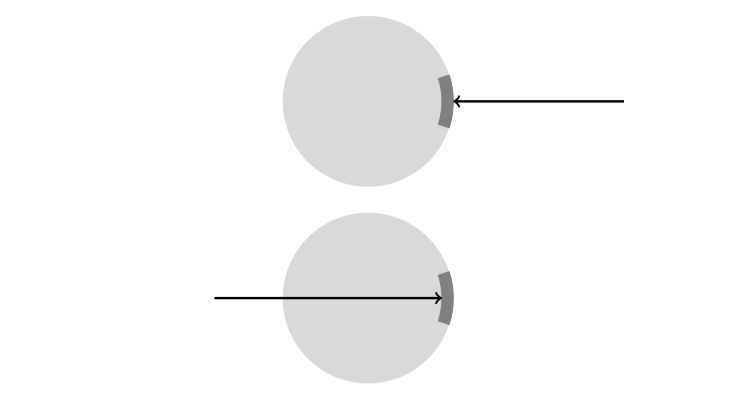
\includegraphics[width=\linewidth]{figures/sph/incoming-outgoing}
  \caption[Angular flux impinged on an FSR]{Angular flux impinged on an FSR from the moderator (top) and after traversing the fuel (bottom). \textit{Image courtesy of N. Gibson~\cite{gibson2016thesis}.}}
\label{fig:chap6-incoming-outgoing}
\end{figure}

A recent PhD thesis by Gibson~\cite{gibson2016thesis} studied the impact of using angular-dependent total \ac{MGXS} on multi-group calculations to avoid the flux separability approximation. Gibson was motivated by his observation of reaction rate errors similar to those discovered in Sec.~\ref{sec:chap5-diagnosis}. In particular, he solved for the reference ultra-fine flux for a 2D \ac{PWR} fuel pin given a fixed source. The reference scalar flux was used to condense the continuous energy total cross sections to 69-group \ac{MGXS}, which were employed in a fixed source transport calculation. The reaction rates computed from the ultra-fine and 69-group scalar fluxes differed by up to 1\% for low-lying energy groups with large U-238 capture resonances, with an error profile in energy similar to that shown in Fig.~\ref{fig:chap5-rel-err-energy}. Gibson's results indicated that an improper treatment of self-shielding effects in heterogeneous geometries may lead to errors in resonant groups even when the exact scalar flux is used to collapse cross sections in energy and space.

Gibson further investigated this issue by using the reference ultra-fine angular flux to compute angular-dependent \ac{MGXS}. Some examples of the angular-dependent capture \ac{MGXS} generated for two different \ac{FSR}s shaded in dark gray are shown in Fig.~\ref{fig:chap6-batman-plots}. The \ac{MGXS} in the \ac{FSR} at the fuel/moderator interface in Fig.~\ref{fig:chap6-batman-plots-a} ranges from less than 5 to more than 50 barns for angles entering and leaving the fuel pin. The peaks near 60$^{\circ}$ and 120$^{\circ}$ are due to extra moderation experienced by neutrons streaming through the infinite rectilinear fuel pin lattice at those angles. The \ac{MGXS} in \ac{FSR}s in the interior of the fuel pin, such as the one shown in Fig.~\ref{fig:chap6-batman-plots-b}, exhibit similar but less prominent properties since the flux is shielded in all directions.

\begin{figure}[h]
\begin{subfigure}{.5\textwidth}
  \centering
  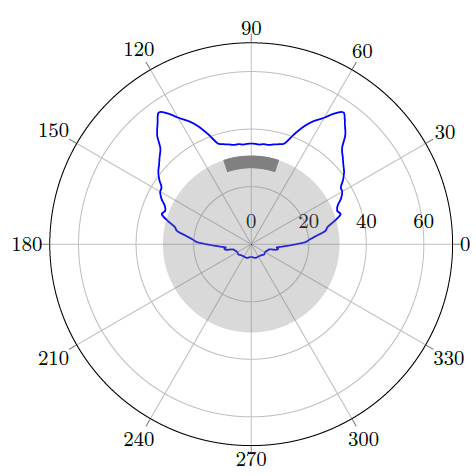
\includegraphics[width=\linewidth]{figures/sph/batman-1}
  \caption{}
  \label{fig:chap6-batman-plots-a}
\end{subfigure}
\begin{subfigure}{.5\textwidth}
  \centering
  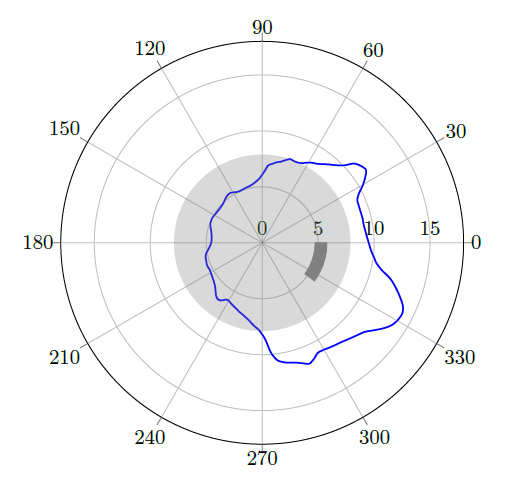
\includegraphics[width=\linewidth]{figures/sph/batman-2}
  \caption{}
  \label{fig:chap6-batman-plots-b}
\end{subfigure}
\caption[Angular-dependent capture MGXS]{Angular-dependent capture \ac{MGXS} for the 6.67 eV resonance group as a function of azimuthal angle for two different \ac{FSR}s. The radial axis is given in units of barns and the azimuthal axis in units of degrees. \textit{Image courtesy of N. Gibson~\cite{gibson2016thesis}.}}
\label{fig:chap6-batman-plots}
\end{figure}

Gibson proceeded to show that the angular-dependent total \ac{MGXS} eliminated the reaction rate errors observed with scalar flux-weighted \ac{MGXS}. His analysis highlighted the tight coupling between angular dependence and spatial discretization. Notably, the reaction rate errors were reduced by an order of magnitude only when angular-dependent \ac{MGXS} were paired with a fine \ac{FSR} spatial discretization. This can be explained by the fact that the angular variation of the volume-integrated flux is diminished as the \ac{FSR} mesh is coarsened. Thus, the spatial self-shielding effects at the fuel/moderator interface cannot be captured by angular-dependent total \ac{MGXS} if the \ac{FSR} discretization is unable to distinguish between neutrons entering and leaving the fuel pin.

Although angular-dependent total \ac{MGXS} the most direct solution to eliminate the flux separability approximation, it is not a desirable approach for a number of reasons. Angular-dependent \ac{MGXS} would significantly increase the memory footprint for \ac{MGXS} libraries, and be complicated to accommodate in multi-group methods. Furthermore, angular-dependent \ac{MGXS} is not attractive for \ac{MC}-based \ac{MGXS} generation since many more particle histories would be required to converge the \ac{MGXS} in each discrete angular tally bin. The Consistent-P approximation~\cite{bell1967transport} is an alternative method that embeds the angular dependence of the total \ac{MGXS} within the angular expansion of the scattering kernel (Eqn.~\ref{eqn:chap2-transport-ce-2}) while retaining an angular independent total \ac{MGXS}. Although the Consistent-P approximation is one viable approach used in many transport codes, it was not evaluated here since anisotropic scattering was not implemented in OpenMOC at the time of this writing. A third method known as SuPerHomog\'{e}n\'{e}isation factors was discussed in this context by Gibson, who employed them to reduce heterogeneous resonant reaction rate errors (albeit to a lesser extent than he achieved with angular-dependent total \ac{MGXS}). \ac{SPH} factors are a relatively simple-to-implement method which do not require an anisotropic scattering kernel implementation. For this reason, the \ac{SPH} factor scheme was evaluated in OpenMOC as discussed in the following sections.

%-Nelson's 1D slab plot(s)?

\begin{emphbox}
\textbf{Multi-group reaction rates are not preserved in heterogeneous geometries due to the flux separability approximation. Angular-dependent total \ac{MGXS} or an equivalence scheme such as \ac{SPH} factors are needed to resolve the bias between OpenMC and OpenMOC.}
\end{emphbox}

%%%%%%%%%%%%%%%%%%%%%%%%%%%%%%%%%%%%%%%%%%%%%%%%%%%%%%%%%%%%%%%%%%%%%%%%%%%%%%%
\section{SuPerHomog\'{e}n\'{e}isation Factors}
\label{sec:chap6-sph}

As discussed in Chap.~\ref{chap:mgxs}, multi-group theory is valid and consistent if and only if \ac{MGXS} are defined to preserve reaction rates. In Chap.~\ref{chap:biases} it was determined that reaction rate preservation is not possible in heterogeneous geometries, even if the exact flux from \ac{MC} is used to collapse the cross sections in energy and space. \ac{SPH} factors were first proposed by H\'{e}bert~\cite{hebert1993consistent} to preserve reaction rates during energy condensation and spatial homogenization. The \ac{SPH} factor algorithm requires knowledge of a reference source that is used in a multi-group fixed source solver to derive multiplicative factors that adjust the total \ac{MGXS} to force neutron balance. 

The literature provides little explanation of the type of approximation errors that \ac{SPH} factors are designed to mitigate. In theory, the \ac{SPH} scheme adjusts \ac{MGXS} to preserve reaction rates irregardless of the source of approximation error -- including errors which derive from a poor treatment of energy and spatial self-shielding, a coarse spatial and angular discretization of the multi-group calculation method, and/or a truncated approximation to the anisotropic scattering kernel. In this section, \ac{SPH} factors are investigated as one approach to resolve the reaction rate errors observed in Chap.~\ref{chap:biases}. The mathematical formulation behind \ac{SPH} factors is described in Sec.~\ref{subsec:chap6-sph-overview}, the iterative algorithm used to compute the factors is summarized in Sec.~\ref{subsec:chap6-sph-algorithm}, and the implementation of \ac{SPH} factors in OpenMOC is highlighted in Sec.~\ref{subsec:chap6-sph-openmoc}.

%%%%%%%%%%%%%%%%%%%%%
\subsection{Overview}
\label{subsec:chap6-sph-overview}

The \ac{SPH} algorithm enforces reaction rate preservation between a reference fine mesh transport problem and a corresponding coarse mesh transport or diffusion problem in energy and space. \ac{SPH} factors have traditionally been applied to spatially-homognenized few-group \ac{MGXS} for coarse mesh diffusion applications. However, this section will introduce \ac{SPH} factors to enforce equivalence between continuous energy Monte Carlo and deterministic multi-group transport methods. 

The \ac{SPH} scheme postulates the existence of a set of factors $\mu_{k,g}$ for each spatial zone $k$ and energy group $g$ which force the streaming and collision terms in the transport equation to balance with a fixed source $Q_{k,g}$:

\begin{dmath}
\label{eqn:chap6-sph-transport-eqn}
\mathbf{\Omega} \cdot \nabla \psi_{g}(\mathbf{r},\mathbf{\Omega}) + \mu_{k,g}\Sigma_{t,k,g}\psi_{g}(\mathbf{r},\mathbf{\Omega}) = Q_{k,g}(\mathbf{\Omega})
\end{dmath}

\noindent In this equation, the \ac{SPH} factors are applied to correct the total \ac{MGXS} in each region and group. The fixed source $Q_{k,g}$ is computed from the reference fine mesh solution. In this case,  the fixed source is treated as the sum of scattering and fission production sources in each energy group and spatial zone. For example, continuous energy Monte Carlo can be used to compute reference multi-group fluxes and \ac{MGXS}, which are then combined to compute an isotropic source as follows:

\begin{dmath}
\label{eqn:chap6-sph-source}
Q_{k,g}(\mathbf{\Omega}) = \frac{1}{4\pi} \sum_{g'=1}^{G} \Sigma_{s,k,g' \rightarrow g}\phi_{k,g'} + \frac{\chi_{k,g}}{4\pi k_{eff}}\sum_{g'=1}^{G} \nu\Sigma_{f,k,g'}\phi_{k,g'}
\end{dmath}

\noindent Given the fixed source and total \ac{MGXS} from \ac{MC}, Eqn.~\ref{eqn:chap6-sph-transport-eqn} may be solved using any multi-group transport method, such as \ac{MOC}. The challenge is to devise estimates to the true \ac{SPH} factors $\mu_{k,g}$ which adequately preserve reaction rates. The following section describes the iterative scheme used to estimate \ac{SPH} factors.

%%%%%%%%%%%%%%%%%%%%%
\subsection{Algorithm}
\label{subsec:chap6-sph-algorithm}

An iterative algorithm is used to estimate \ac{SPH} factors from a series of multi-group fixed source calculations. First, the estimates $\mu_{k,g}^{(n)}$ at iteration $n$ to the true \ac{SPH} factors $\mu_{k,g}$ are introduced as a correction factor for the total cross section in Eqn.~\ref{eqn:chap6-sph-transport-eqn}:

\begin{dmath}
\label{eqn:chap6-sph-transport-eqn-iterate}
\mathbf{\Omega} \cdot \nabla \psi_{g}^{(n)}(\mathbf{r},\mathbf{\Omega}) + \mu_{k,g}^{(n-1)}\Sigma_{t,k,g}\psi_{g}^{(n)}(\mathbf{r},\mathbf{\Omega}) = Q_{k,g}(\mathbf{\Omega})
\end{dmath}

\noindent This form of the transport equation with a fixed source is solved using a multi-group transport code (such as OpenMOC) for the flux distribution at each iteration. The \ac{SPH} factor estimates $\mu_{k,g}^{(n)}$ are found from the ratio of the reference Monte Carlo scalar flux $\phi_{k,g}^{MC}$ to the flux $\phi_{k,g}^{(n)}$ computed from the fixed source calculation at iteration $n$,

\begin{equation}
\label{eqn:chap6-sph-update}
\mu_{k,g}^{(n)} = \frac{\phi_{k,g}^{MC}}{\phi_{k,g}^{(n)}}
\end{equation}

\noindent where the factors are initialized to unity on the first iteration:

\begin{dmath}
\label{eqn:chap6-sph-initial}
\mu_{k,g}^{(0)} = 1
\end{dmath}

The \ac{SPH} factors are used to find a total \ac{MGXS} which forces neutron balance in Eqn.~\ref{eqn:chap6-sph-transport-eqn-iterate}. The initial total \ac{MGXS} $\Sigma_{t,k,g}^{(0)}$ is computed from the reference \ac{MC} flux and total reaction rate tallies. The \ac{SPH} factors are then used to obtain a corrected total \ac{MGXS} $\Sigma_{t,k,g}^{(n)}$ on each iteration:

\begin{dmath}
\label{eqn:chap6-sph-update-sigt}
\Sigma_{t,k,g}^{(n)} = \mu_{k,g}^{(n-1)}\Sigma_{t,k,g}^{(0)}
\end{dmath}

The series of fixed source problems defined by Eqn.~\ref{eqn:chap6-sph-transport-eqn-iterate} are solved until the \ac{SPH} factors converge. A common convergence criterion is the maximum relative absolute deviation across energy groups and spatial zones:

\begin{dmath}
\label{eqn:chap6-sph-residual}
res = \max_{k,g} \left|\frac{\mu_{k,g}^{(n)} - \mu_{k,g}^{(n-1)}}{\mu_{k,g}^{(n-1)}}\right|
\end{dmath}

\noindent A residual of 10$_{-7}$ can typically be achieved with twenty or fewer iterations.

The scattering matrix $\Sigma_{s,k,g'\rightarrow g}$ and fission production cross section $\nu\Sigma_{f,k,g}$ are used to compute the reference fixed source in Eqn.~\ref{eqn:chap6-sph-source}, but are not needed in the iterative scheme defined in Eqn.~\ref{eqn:chap6-sph-transport-eqn-iterate}. However, in the context of this thesis, \ac{SPH} factors are computed to preserve reaction rates in subsequent eigenvalue calculations. Therefore, the \ac{SPH} factors must be applied to the scattering matrix and fission production cross sections to produce a fully-corrected \ac{MGXS} library:

\begin{dmath}
\label{eqn:chap6-sph-update-sigs}
\Sigma_{s,k,g'\rightarrow g}^{(n)} = \mu_{k,g}^{(n-1)}\Sigma_{s,k,g'\rightarrow g}^{(0)}
\end{dmath}

\begin{dmath}
\label{eqn:chap6-sph-update-nusigf}
\nu\Sigma_{f,k,g}^{(n)} = \mu_{k,g}^{(n-1)}\nu\Sigma_{f,k,g}^{(0)}
\end{dmath}

It should be noted that although the \ac{SPH}-corrected \ac{MGXS} are defined to preserve reaction rates, they will not preserve the group-wise scalar flux. However, the angular or scalar flux may be easily recovered from the fluxes $\tilde{\psi}_{k,g}$ and $\tilde{\phi}_{k,g}$ computed with the \ac{SPH}-corrected \ac{MGXS} in an eigenvalue or fixed source calculation:

\begin{dmath}
\label{eqn:chap6-sph-update-angular-flux}
\psi_{k,g} = \mu_{k,g}\tilde{\psi}_{k,g}
\end{dmath}

\begin{dmath}
\label{eqn:chap6-sph-update-scalar-flux}
\phi_{k,g}^{(n)} = \mu_{k,g}\tilde{\phi}_{k,g}
\end{dmath}

The \ac{SPH} iteration algorithm described here is summarized in Alg.~\ref{alg:chap6-sph}. It should be noted that as presently posed, there is no unique solution to the set of \ac{SPH} factors which preserve reaction rates. A unique solution may be found by forcing the factors to be unity in non-fissile zones (\textit{e.g.}, moderator, clad and gap). This approach is motivated by the fact that resonances which lead to self-shielding errors -- such as the U-238 capture resonances studied in Sec.~\ref{subsec:chap2-angle} -- are generally from isotopes in the fuel. However, the reaction rates in non-fissile zones will not be preserved since the \ac{MGXS} in these zones remain uncorrected, but these errors are likely dominated by those in the fuel as was shown for the \ac{PWR} benchmarks in Sec.~\ref{subsec:chap5-diagnosis-rxn-rates}.

\begin{algorithm}[h]
\caption{SPH Factor Algorithm}
\label{alg:chap6-sph}
\begin{algorithmic}[1]
  \State Initialize $\Sigma_{t,k,g}^{(0)}$, $\Sigma_{s,k,g'\rightarrow g}^{(0)}$, $\nu\Sigma_{f,k,g}^{(0)}$, and $\chi_{k,g}^{(0)}$ from MC tallies \Comment{Tab.~\ref{table:chap3-tally-types}}
  \State Compute $Q_{k,g}$ from MC flux and \ac{MGXS} \Comment{Eqn.~\ref{eqn:chap6-sph-source}}
  \State Initialize $\mu_{k,g}^{(0)}$ to unity
  \While{SPH factor residuals are not converged}
    \State Update $\Sigma_{t,k,g}^{(n)}$ with \ac{SPH} factors \Comment{Eqn.~\ref{eqn:chap6-sph-update-sigt}}
    \State Solve fixed source transport problem\footnotemark \Comment{Eqn.~\ref{eqn:chap6-sph-transport-eqn-iterate}}
    \State Compute new \ac{SPH} factors $\mu_{k,g}^{(n)}$ \Comment{Eqn.~\ref{eqn:chap6-sph-update}}
    \State Compute \ac{SPH} factor residuals \Comment{Eqn.~\ref{eqn:chap6-sph-residual}}
  \EndWhile
  \State Compute final \ac{MGXS} with \ac{SPH} factors \Comment{Eqns.~\ref{eqn:chap6-sph-update-sigt},~\ref{eqn:chap6-sph-update-sigs},~\ref{eqn:chap6-sph-update-nusigf}}
\end{algorithmic}
\end{algorithm}

\footnotetext{A series of $G$ independent fixed source problems may be solved for each of the $G$ groups. Alternatively, a single fixed source problem may simultaneously solve for all $G$ groups, as is done in OpenMOC.}

%%%%%%%%%%%%%%%%%%%%%%%%%%%%%%%%%%%%%%
\subsection{Implementation in OpenMOC}
\label{subsec:chap6-sph-openmoc}

The \ac{SPH} scheme was implemented in the \texttt{openmoc.materialize} Python module of the OpenMOC code (see Sec.~\ref{subsubsec:chap4-openmoc-mgxs}). The \ac{SPH} algorithm was specifically implemented to work with the \texttt{Library} class included in the \texttt{openmc.mgxs} Python module for \ac{MGXS} generation with OpenMC (see Sec.~\ref{subsec:chap4-mgxs}). In particular, the fixed source in Eqn.~\ref{eqn:chap6-sph-source} is computed from the \ac{MC} tallies in the \texttt{Library} object and used to construct a fixed source simulation in OpenMOC. The \ac{MGXS} tabulated in the \texttt{Library} are loaded into OpenMOC, and the series of fixed source calculations in Alg.~\ref{alg:chap6-sph} is managed from Python. The \ac{MGXS} data in the \texttt{Library} is updated with the \ac{SPH} factors computed at each iteration. The final corrected \ac{MGXS} \texttt{Library}, along with the \ac{SPH} factors, are returned to the user for use in subsequent OpenMOC eigenvalue calculations.

Although the \ac{SPH} algorithm is relatively simple, a few subtle issues made the implementation in OpenMOC less than straightforward. First, it should be noted that OpenMC tallies are volume-integrated, while reaction rates and fluxes in OpenMOC are volume-averaged. As a result, the \ac{MC} tallies must be normalized to the volume used by OpenMOC for each \ac{FSR} as opposed to the true volumes\footnote{OpenMOC estimates spatial volumes by integrating the characteristic track lengths across each \ac{FSR}.} to calculate the volume-averaged fixed source in each \ac{FSR}. In addition, it was relatively complicated to map the \ac{MGXS} data and \ac{SPH} factors between the combinatorial geometry meshes used by OpenMC and OpenMOC. These challenges notwithstanding, \ac{SPH} factors were implemented in OpenMOC v0.2.1, and used to reduce reaction rate errors as discussed in the following section.

\begin{emphbox}
\textbf{The \ac{SPH} factor approach uses a reference fixed source to correct the total \ac{MGXS} to preserve reaction rates between fine and coarse mesh methods.}
\end{emphbox}

%%%%%%%%%%%%%%%%%%%%%%%%%%%%%%%%%%%%%%%%%%%%%%%%%%%%%%%%%%%%%%%%%%%%%%%%%%%%%%%
\section{Case Studies}
\label{sec:chap6-sph-case-studies}

A number of case studies were performed to evaluate the effectiveness of \ac{SPH} factors in eliminating the bias observed between OpenMC and OpenMOC in Chap.~\ref{chap:biases}. The 1D slab and 2D fuel pin benchmarks described in Secs.~\ref{subsec:chap5-slab} and~\ref{subsec:chap5-pin}, respectively, were modeled with \ac{SPH}-corrected \ac{MGXS} for the \ac{FSR}s in the fuel and compared to the original results. The \ac{MGXS} were computed using isotropic in lab scattering and a spatial tally mesh corresponding to the \ac{FSR} mesh (see Tabs.~\ref{table:chap5-slab-space} and~\ref{table:chap5-pin-space}). The OpenMOC fixed source and eigenvalue calculations were performed with 128 azimuthal angles and 0.01 cm track spacing. The OpenMOC fixed source calculations were converged to 10$_{-5}$ on the average \ac{FSR} scalar flux. A convergence criterion of 10$_{-7}$ was used to converge the \ac{SPH} factors in Eqn.~\ref{eqn:chap6-sph-residual}. Finally, the energy-integrated \ac{FSR} fission source was converged to 10$_{-7}$ in the eigenvalue calculations with \ac{SPH}-corrected \ac{MGXS}.

The eigenvalue bias for the 1D slab and 2D fuel pin with \ac{SPH}-corrected \ac{MGXS} are presented in Sec.~\ref{subsubsec:chap6-sph-eigenvalues}. The error profiles of the energy-dependent and spatially-dependent fluxes within the fuel \ac{FSR}s, as well as the \ac{SPH} factors in energy and space, are analyzed in Secs.~\ref{subsec:chap6-sph-flux-energy} and~\ref{subsec:chap6-sph-flux-space}, respectively.

%%%%%%%%%%%%%%%%%%%%%%%%%%%%%%%%%%%%%%
\subsection{Impact of SPH on Eigenvalues}
\label{subsubsec:chap6-sph-eigenvalues}

The first case study compared the eigenvalues computed with and without \ac{SPH} factors. The eigenvalue bias $\Delta\rho$ between OpenMC and OpenMOC is presented for a matrix of energy group structures and \ac{FSR} discretization in Tabs.~\ref{table:chap6-sph-slab-energy} and~\ref{table:chap6-sph-pin-energy} for a 1D slab and 2D fuel pin, respectively. The bias without \ac{SPH} factors is reproduced from Tabs.~\ref{table:chap5-slab-space} and~\ref{table:chap5-pin-space} for comparison purposes.

The data in the tables illustrate a large reduction in the eigenvalue bias with \ac{SPH}-corrected \ac{MGXS}. With only a few exceptions, the bias is consistently positive and ranges between 10 -- 40 \ac{pcm} for both geometries. In the case of the slab, the bias of -93 \ac{pcm} with the finest energy group structure and \ac{FSR} discretization was reduced by a factor of 7$\times$ to only 13 \ac{pcm} with \ac{SPH}-corrected \ac{MGXS}. The use of \ac{SPH} factors had an even greater impact on the bias for the fuel pin, where the bias of over -211 \ac{pcm} was reduced by 70$\times$ to just -3 \ac{pcm} for the finest energy and spatial discretization. 

Although these results illustrate much better agreement between OpenMC and OpenMOC, it is interesting to note that a non-neglible bias remains in most cases. As was noted in Sec.~\ref{subsec:chap6-sph-algorithm}, the reaction rates in non-fissile zones such as the moderator are not preserved with \ac{SPH} which may contribute to the lingering eigenvalue bias. In addition, the remaining bias may be due to the fact that the reaction rate balance enforced with \ac{SPH} factors assumes that the eigenvalue calculation with a multi-group method will produce the same neutron source distribution as \ac{MC}. However, the eigenvalue source is not necessarily conserved since approximation errors from spatial and angular discretization will impact the multi-group method's solution. In conclusion, the eigenvalues between OpenMC and OpenMOC will identically match if and only if OpenMOC computes precisely the same eigenvalue source with \ac{SPH}-corrected \ac{MGXS} as that found by OpenMC.

\begin{table}[h!]
  \centering
  \caption[Eigenvalues with SPH factors for a 1D slab]{The impact of SPH factors on the eigenvalue bias $\Delta\rho$ with varying energy group structures and \ac{FSR} spatial discretizations for a 1D slab.}  
  \label{table:chap6-sph-slab-energy}
  \vspace{6pt}
  \begin{tabular}{| q | S[table-format=6.1] S[table-format=6.1] S[table-format=6.1] S[table-format=6.1] S[table-format=6.1] |}
  \hhline{~|-----|}
  \multicolumn{1}{c|}{\cellcolor{white}} & \multicolumn{5}{c|}{\cellcolor{lightgray} {\bf \ac{FSR} Discretization}} \\
  \multicolumn{1}{c|}{\cellcolor{white}} &
  {\cellcolor{lightgray} {\bf 1$\times$}} &
  {\cellcolor{lightgray} {\bf 2$\times$}} &
  {\cellcolor{lightgray} {\bf 4$\times$}} &
  {\cellcolor{lightgray} {\bf 8$\times$}} &
  {\cellcolor{lightgray} {\bf 16$\times$}} \\
  \midrule
  \multicolumn{1}{|c|}{\cellcolor{lightgray} {\bf \# Groups}} & \multicolumn{5}{c|}{\cellcolor{carolinablue} \bf Without SPH} \\
  \hhline{~|-----|}
1 & 139 & 97 & 127 & 162 & 140 \\
2 & 296 & 145 & 100 & 90 & 88 \\
4 & 233 & 125 & 77 & 61 & 51 \\
8 & 304 & 136 & 45 & 7 & -9 \\
16 & 329 & 139 & 38 & -6 & -23 \\
25 & 266 & 83 & -11 & -54 & -70 \\
40 & 270 & 75 & -29 & -73 & -89 \\
70 & 280 & 76 & -33 & -81 & {\cellcolor{darktangerine}} -93 \\
  \midrule
  \multicolumn{1}{c|}{\cellcolor{white}} & \multicolumn{5}{c|}{\cellcolor{lightgreen} \bf With SPH} \\
  \midrule
1 & 33 & -10 & 18 & 51 & 30 \\
2 & 36 & 13 & 27 & 34 & 16 \\
4 & 18 & 26 & 28 & 33 & 18 \\
8 & 27 & 37 & 29 & 22 & 12 \\
16 & 27 & 38 & 30 & 20 & 9 \\
25 & 28 & 39 & 34 & 25 & 12 \\
40 & 28 & 39 & 31 & 23 & 12 \\
70 & 31 & 41 & 31 & 20 & {\cellcolor{darktangerine}} 13 \\
  \bottomrule
\end{tabular}
\end{table}

\begin{table}[h!]
  \centering
  \caption[Eigenvalues with SPH factors for a 2D fuel pin]{The impact of SPH factors on the eigenvalue bias $\Delta\rho$ with varying energy group structures and \ac{FSR} spatial discretizations for a 2D fuel pin.}
  \label{table:chap6-sph-pin-energy} 
  \vspace{6pt}
  \begin{tabular}{| q | S[table-format=6.1] S[table-format=6.1] S[table-format=6.1] S[table-format=6.1] S[table-format=6.1] |}
  \hhline{~|-----|}
  \multicolumn{1}{c|}{\cellcolor{white}} & \multicolumn{5}{c|}{\cellcolor{lightgray} {\bf \ac{FSR} Discretization}} \\
  \multicolumn{1}{c|}{\cellcolor{white}} &
  {\cellcolor{lightgray} {\bf 1$\times$}} &
  {\cellcolor{lightgray} {\bf 2$\times$}} &
  {\cellcolor{lightgray} {\bf 4$\times$}} &
  {\cellcolor{lightgray} {\bf 8$\times$}} &
  {\cellcolor{lightgray} {\bf 16$\times$}} \\
  \midrule
  \multicolumn{1}{|c|}{\cellcolor{lightgray} {\bf \# Groups}} & \multicolumn{5}{c|}{\cellcolor{carolinablue} \bf Without SPH} \\
  \hhline{~|-----|}
1 & 80 & 92 & 55 & 83 & 66 \\
2 & 141 & 87 & 29 & 50 & 34 \\
4 & 27 & -15 & -43 & -45 & -57 \\
8 & 26 & -34 & -85 & -90 & -102 \\
16 & 35 & -35 & -91 & -101 & -111 \\
25 & -31 & -105 & -158 & -170 & -182 \\
40 & -38 & -114 & -174 & -189 & -202 \\
70 & -39 & -117 & -182 & -196 & {\cellcolor{darktangerine}} -211 \\
  \midrule
  \multicolumn{1}{c|}{\cellcolor{white}} & \multicolumn{5}{c|}{\cellcolor{lightgreen} \bf With SPH} \\
  \midrule
1 & 19 & 25 & -18 & 10 & -14 \\
2 & 25 & 20 & -14 & 18 & -6 \\
4 & 7 & 10 & 2 & 12 & 1 \\
8 & 4 & 13 & -0 & 12 & 2 \\
16 & 5 & 13 & 0 & 10 & 4 \\
25 & 5 & 13 & 2 & 12 & -1 \\
40 & 4 & 16 & 3 & 11 & -2 \\
70 & 4 & 17 & 2 & 12 & {\cellcolor{darktangerine}} -3 \\
  \bottomrule
\end{tabular}
\end{table}

%%%%%%%%%%%%%%%%%%%%%%%%%%%%%%%%%%%%%%%%%%%%%%%%
\subsection{Impact of SPH on the Energy-Dependent Flux}
\label{subsec:chap6-sph-flux-energy}
%\subsection{SPH Factors in Energy}
%\label{subsubsec:chap6-sph-energy}

A second case study investigated the impact of \ac{SPH} factors on the energy-dependent flux errors identified in Sec.~\ref{subsec:chap5-diagnosis-energy}. The error of OpenMOC's 70-group flux with respect to the reference OpenMC flux is displayed in Fig.~\ref{fig:chap6-rel-err-energy} for the slab and pin. The errors are shown for the innermost and outermost \ac{FSR}s in the fuel. The flux errors without \ac{SPH}-corrected \ac{MGXS} are reproduced from Fig.~\ref{fig:chap5-rel-err-energy} and are illustrated with dashed lines for comparison purposes. 

\begin{figure}[h!]
\begin{subfigure}{.9\textwidth}
  \centering
  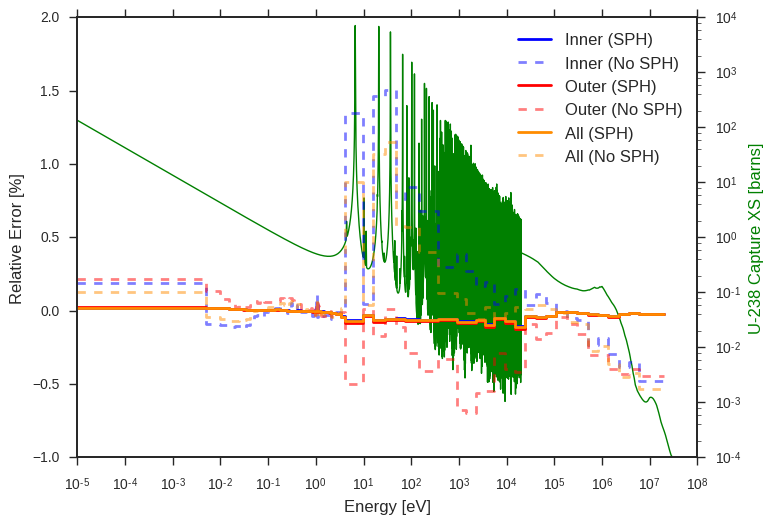
\includegraphics[width=\linewidth]{figures/sph/slab/rel-err-inner-outer}
  \caption{}
\end{subfigure}
\begin{subfigure}{.9\textwidth}
  \centering
  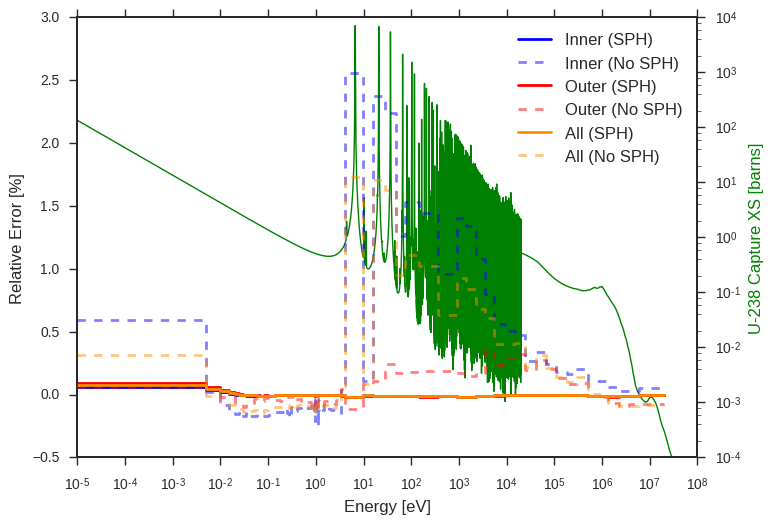
\includegraphics[width=\linewidth]{figures/sph/pin-cell/rel-err-inner-outer}
  \caption{}
\end{subfigure}
\caption[Flux relative error by energy group w/ SPH]{The energy-dependent relative error of the 70-group OpenMOC scalar flux with respect to the reference OpenMC flux in a 1D slab (a) and 2D fuel pin (b). The results correspond to Tables~\ref{table:chap6-sph-slab-energy} and~\ref{table:chap6-sph-pin-energy}.}
\label{fig:chap6-rel-err-energy}
\end{figure}

\begin{figure}[h!]
\begin{subfigure}{.9\textwidth}
  \centering
  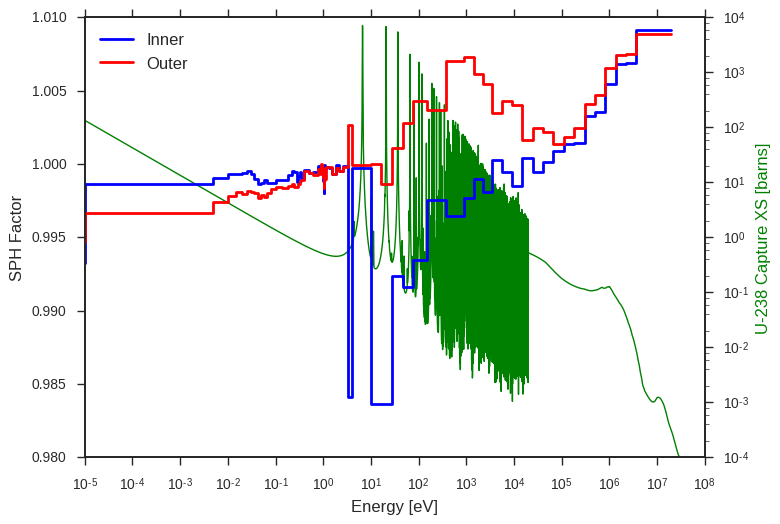
\includegraphics[width=\linewidth]{figures/sph/slab/sph-inner-outer}
  \caption{}
\end{subfigure}
\begin{subfigure}{.9\textwidth}
  \centering
  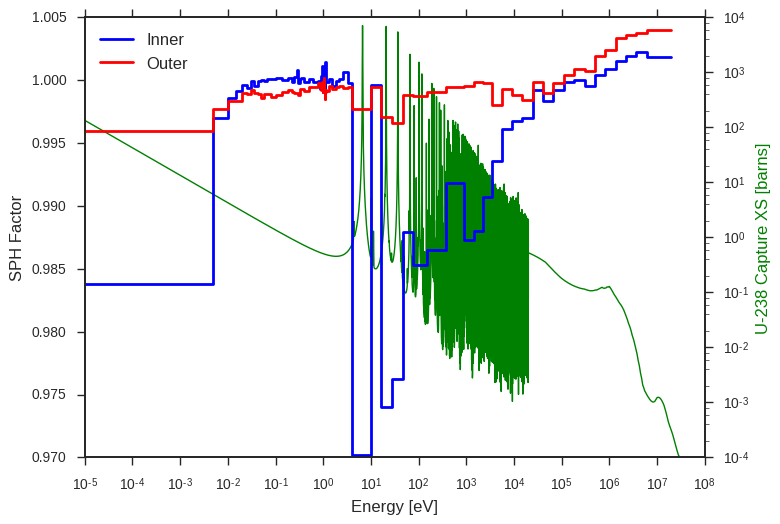
\includegraphics[width=\linewidth]{figures/sph/pin-cell/sph-inner-outer}
  \caption{}
\end{subfigure}
\caption[SPH factors by energy group]{The energy-dependent \ac{SPH} factors for a 70-group calculation in a 1D slab (a) and 2D fuel pin (b). The results correspond to Tables~\ref{table:chap6-sph-slab-energy} and~\ref{table:chap6-sph-pin-energy}.}
\label{fig:chap6-sph-energy}
\end{figure}

As expected, the flux error is greatly reduced with \ac{SPH}-corrected \ac{MGXS}. The flux error profile is nearly flat in energy for both innermost and outermost \ac{FSR}s, unlike the highly energy-dependent profiles observed without \ac{SPH}. Furthermore, no systematic difference between the error profiles for the innermost and outermost \ac{FSR}s can be discerned from the plots. The improvement in OpenMOC's flux -- especially in those energy groups with large U-238 capture resonances -- is responsible for the reduction in the eigenvalue bias with \ac{SPH}-corrected \ac{MGXS} presented in Sec.~\ref{subsubsec:chap6-sph-eigenvalues}.

The \ac{SPH} factors in each energy group are illustrated for the innermost and outermost \ac{FSR}s in the slab and pin in Fig.~\ref{fig:chap6-sph-energy}. The \ac{SPH} factors show nearly the opposite energy-dependent behavior of the flux errors without \ac{SPH} factors. In general, the factors are less than unity in those groups with positive flux errors (\textit{e.g.}, the fast groups), while the factors are greater than unity in groups with negative errors (\textit{e.g.}, resonance groups in the innermost \ac{FSR}). This behavior is expected since an \ac{SPH} factor greater than unity will magnify the total cross section (see Eqn.~\ref{eqn:chap6-sph-update-sigt}) which will reduce the scalar flux, and vice versa. Furthermore, the deviation of the \ac{SPH} factors from unity is roughly the same as the error in each respective group. For example, the flux in group 27 with the U-238 capture resonance at 6.67 eV exhibits an error of nearly 1.5\% and 2.5\% for the slab and pin, respectively. Similarly, the \ac{SPH} factors in group 27 are approximately 0.984 and 0.970, or 1.6\% and 3\% reduced from unity, for the slab and pin.

%%%%%%%%%%%%%%%%%%%%%%%%%%%%%%%%%%%%%%%%%%%%%%%%%%%
\subsection{Impact of SPH on the Spatially-Dependent Flux}
\label{subsec:chap6-sph-flux-space}
%\subsection{SPH Factors in Space}
%\label{subsubsec:chap6-sph-space}

A final case study investigated the impact of \ac{SPH} factors on the spatially-dependent 70-group flux errors identified in Sec.~\ref{subsec:chap5-diagnosis-space}. The error of OpenMOC's flux with respect to the reference OpenMC flux is displayed in Fig.~\ref{fig:chap6-rel-err-space} for the slab and pin. The errors are shown for group 27 for each of the \ac{FSR}s in the fuel. This plot can be compared to the spatially-dependent errors in Fig.~\ref{fig:chap5-rel-err-space} observed without \ac{SPH}-corrected \ac{MGXS}.

\begin{figure}[h!]
\begin{subfigure}{.9\textwidth}
  \centering
  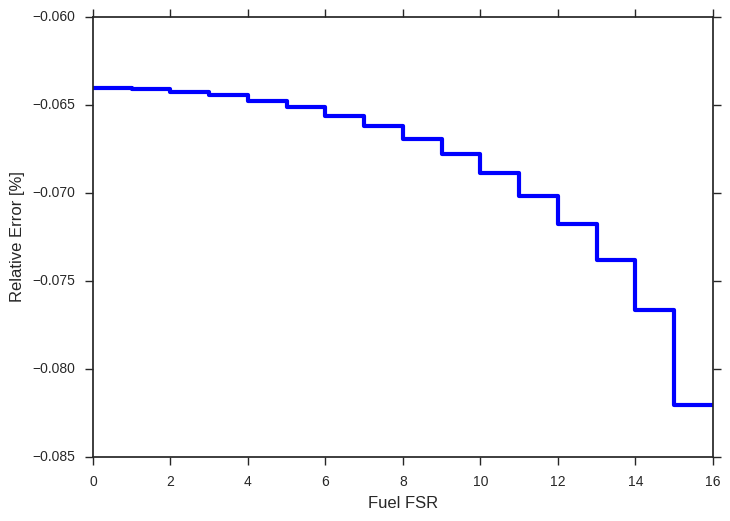
\includegraphics[width=0.9\linewidth]{figures/sph/slab/rel-err-fuel-fsrs}
  \caption{}
\end{subfigure}
\begin{subfigure}{.9\textwidth}
  \centering
  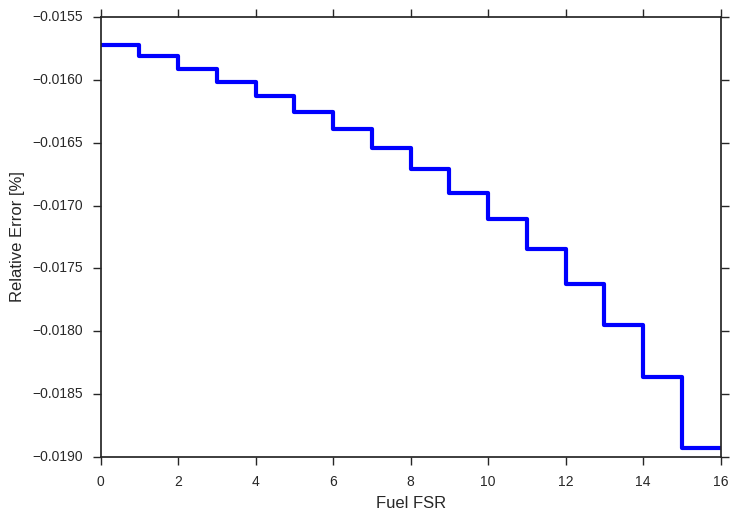
\includegraphics[width=0.9\linewidth]{figures/sph/pin-cell/rel-err-fuel-fsrs}
  \caption{}
\end{subfigure}
\caption[Flux relative error by FSR w/ SPH]{The spatially-varying relative error of the OpenMOC scalar flux with respect to the reference OpenMC flux for a 1D slab (a) and 2D fuel pin (b) in group 27. The results correspond to Tables~\ref{table:chap6-sph-slab-energy} and~\ref{table:chap6-sph-pin-energy}.}
\label{fig:chap6-rel-err-space}
\end{figure}

\begin{figure}[h!]
\begin{subfigure}{.9\textwidth}
  \centering
  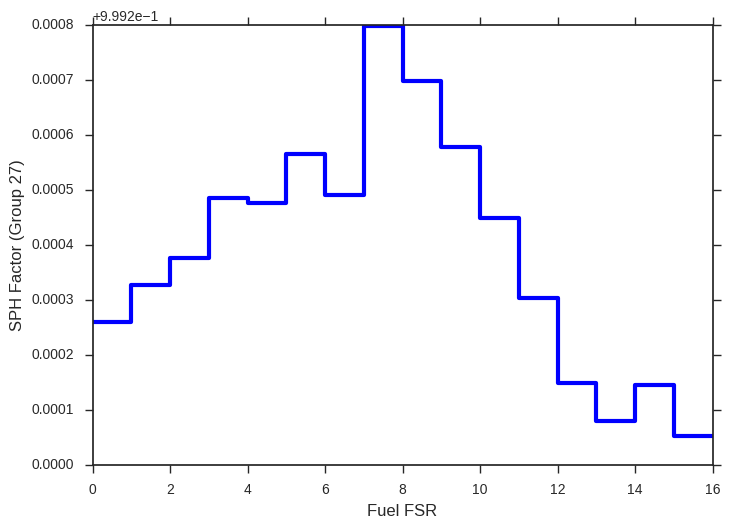
\includegraphics[width=0.9\linewidth]{figures/sph/slab/sph-fuel-fsrs}
  \caption{}
\end{subfigure}
\begin{subfigure}{.9\textwidth}
  \centering
  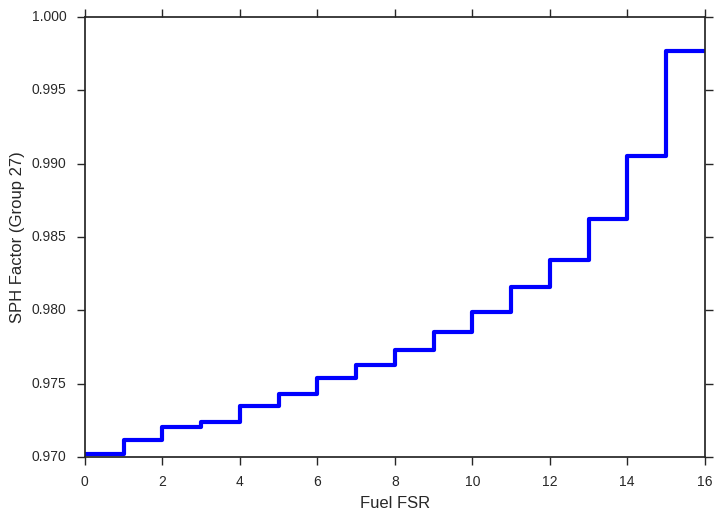
\includegraphics[width=0.9\linewidth]{figures/sph/pin-cell/sph-fuel-fsrs}
  \caption{}
\end{subfigure}
\caption[SPH factors by FSR]{The spatially-varying \ac{SPH} factors for a 1D slab (a) and 2D fuel pin (b) in group 27. The results correspond to Tables~\ref{table:chap6-sph-slab-energy} and~\ref{table:chap6-sph-pin-energy}.}
\label{fig:chap6-sph-space}
\end{figure}

As expected, the flux error in all of the fuel \ac{FSR}s is greatly reduced with the application of \ac{SPH} factors. The maximum errors of approximately -0.082\% and -0.019\% with \ac{SPH} compare to 1.3\% and 2.5\% without \ac{SPH} for the slab and pin, respectively. The overall error profile as plotted appears similar in shape to the case without \ac{SPH} factors in Fig.~\ref{fig:chap5-rel-err-space}, though the fractional variation of the errors is far smaller with \ac{SPH}. Interestingly, the errors with \ac{SPH} are greatest in magnitude in the outermost \ac{FSR}s nearest to the moderator. In contrast, the errors are greatest in magnitude in the innermost \ac{FSR}s furthest removed from the moderator for the case without \ac{SPH} factors. The reduction in the error across the fuel in group 27 is largely responsible for the reduction in the eigenvalue bias with \ac{SPH}-corrected \ac{MGXS} presented in Sec.~\ref{subsubsec:chap6-sph-eigenvalues}.

The group 27 \ac{SPH} factors in each of the \ac{FSR}s in the fuel is illustrated in Fig.~\ref{fig:chap6-sph-space}. The \ac{SPH} factors show nearly the opposite spatially-dependent behavior of the flux errors without \ac{SPH} factors. As discussed in Sec.~\ref{subsec:chap6-sph-flux-energy}, the factors are less than unity in those \ac{FSR}s with positive flux errors, while the factors are greater than unity in groups with negative errors (\textit{e.g.}, the outermost ring in the fuel pin). This behavior is expected since an \ac{SPH} factor greater than unity will magnify the total cross section (see Eqn.~\ref{eqn:chap6-sph-update-sigt}) which will reduce the scalar flux, and vice versa. Furthermore, the deviation of the \ac{SPH} factors from unity is roughly the same as the error in each respective group. For example, the flux in the innermost \ac{FSR} exhibits an error of nearly 1.5\% and 2.5\% for the slab and pin, respectively. Similarly, the \ac{SPH} factors in the innermost \ac{FSR}s are approximately 0.984 and 0.970, or 1.6\% and 3\% reduced from unity, for the slab and pin.

\begin{emphbox}
\textbf{The flux errors in the resonance groups, and the resulting eigenvalue bias between OpenMC and OpenMOC, is largely resolved with \ac{SPH} factors.}
\end{emphbox}

%%%%%%%%%%%%%%%%%%%%%%%%%%%%%%%%%%%%%%%%%%%
%\subsection{2D Heterogeneous Fuel Assembly}
%\label{subsec:chap6-sph-hetero-lat}

%\begin{itemize}[noitemsep]
%  \begin{itemize}[noitemsep]
%    \item cell-avg SPH, region-avg SPH, region-clustered (LNS?) SPH
%  \end{itemize}
%  \item bar chart / rug plot of SPH factors in resonance group(s)
%\end{itemize}

%%%%%%%%%%%%%%%%%%%%%%%%%%%%%%%%%%%%%%%%%%%%%%%%%%%%%%%%%%%%%%%%%%%%%%%%%%%%%%%
\section{Shortcomings of SPH Factors}
\label{sec:chap6-sph-shortcomings}

This chapter identified the flux separability approximation as the culprit in the bias observed between OpenMC and OpenMOC for simple heterogeneous benchmarks in Chap.~\ref{chap:biases}. The \ac{SPH} factor approach was introduced as one method to force reaction rate preservation in multi-group methods with \ac{MGXS} generated from Monte Carlo. Although the use of \ac{SPH} factors was demonstrated to greatly improve the agreement between OpenMC and OpenMOC in Sec.~\ref{sec:chap6-sph-case-studies}, the \ac{SPH} approach suffers from a number of shortcomings which may preclude it from further use in this setting in the future. In particular, the \ac{SPH} scheme requires knowledge of the reference source distribution, is dependent on the spatial discretization mesh, and is indiscriminate between various sources of approximation error.

Perhaps the most significant weakness of the \ac{SPH} approach in the context of \ac{MC}-generated \ac{MGXS} is that it requires knowledge of the true eigenvalue source distribution. The goal of generating \ac{MGXS} with \ac{MC} is to enable multi-group methods to accurately solve eigenvalue problems for the source and flux distributions. If a reference source must first be computed with \ac{MC} in order to compute \ac{SPH}-corrected \ac{MGXS}, then there is no reason to perform a subsequent multi-group calculation since the solution is already known from \ac{MC}.

Furthermore, the \ac{SPH} scheme is wholly dependent on the spatial discretization used by downstream deterministic multi-group methods. In particular, the reference source in Eqn.~\ref{eqn:chap6-sph-source} must be calculated from \ac{MC} tallies in each of the spatial mesh cells used by the \ac{SPH} iteration scheme. In the implementation presented here, the reference source must be computed from OpenMC tallies for each of the \ac{FSR}s in the OpenMOC eigenvalue calculation. This is problematic since a finer \ac{FSR} discretization will potentially require more particle histories to converge the tallies needed to compute the reference source on the finer spatial tally mesh.

Finally, the \ac{SPH} scheme attempts to preserve reaction rates between OpenMC and OpenMOC irregardless of the types of approximation errors which may lead to bias between the two codes. This chapter used \ac{SPH} factors to mitigate the errors due to the flux separability approximation. However, the \ac{SPH} scheme simultaneously attempts to also ``correct'' the \ac{MGXS} to account for spatial, angular and energy discretization errors, approximation error due to the treatment of the scattering kernel, and/or any other approximation error inherent in multi-group methods. For example, the results presented in Sec.~\ref{subsubsec:chap6-sph-eigenvalues} illustrated a broadly consistent agreement between OpenMC and OpenMOC eigenvalues for all energy group structures and \ac{FSR} discretizations, even though systematic trends in the bias were observed in both energy and space without \ac{SPH} factors. This highlights the fact that \ac{SPH} ``corrected'' for not only the lack of angular dependence in the total \ac{MGXS}, but also errors inherent to the energy group structures and \ac{FSR} discretizations. As a result, the same discretization parameters must be used in both the fixed source calculations in the \ac{SPH} iteration scheme, as well as subsequent eigenvalue calculations with \ac{SPH}-corrected \ac{MGXS}\footnote{For OpenMOC, the same number of azimuthal angles, track spacing and \ac{FSR} discretization must be used in both the \ac{SPH} factor and eigenvalue calculations.}.

\clearpage

\begin{emphbox}
\textbf{The \ac{SPH} factor approach is complicated by the need to compute a reference fixed source with \ac{MC} for the spatial discretization mesh used in multi-group methods. In addition, \ac{SPH} factors do not simply correct for the error due to the flux separability approximation, but instead indiscriminately correct for all sources of approximation error between \ac{MC} and multi-group methods.}
\end{emphbox}

%%%%%%%%%%%%%%%%%%%%%%%%%%%%%%%%%%%%%%%%%%%%%%%%%%%%%%%%%%%%%%%%%%%%%%%%%%%%%%%
\section{Future Work}
\label{sec:chap6-sph-future}

As a result of the shortcomings to the \ac{SPH} approach, it is unclear whether the \ac{SPH} factors may broadly applied to correct for the flux separability approximation in \ac{MGXS} generated from \ac{MC}. Future work should investigate whether a universal set of \ac{SPH} factors may be tabulated for known geometries (\textit{e.g.}, \ac{PWR} fuel pins). For example, if the \ac{SPH} factors in the resonance groups are relatively invariant to the fuel enrichment, moderator density, burnup, neighboring pin types, etc. then a single set of \ac{SPH} factors may be computed for an infinite pin cell and applied to each fuel pin in heterogeneous \ac{PWR} lattice and whole-core calculations. 

Although it may be possible to universally apply pre-tabulated \ac{SPH} factors to fixed geometric configurations, it will likely be necessary to develop alternative methods to account for the angular dependence of the total \ac{MGXS}. For example, the angular dependence of the total \ac{MGXS} may be adequately embedded into the scattering kernel using the Consistent-P approximation~\cite{bell1967transport} (also known as the BHS approximation). Alternatively, a coarse set of angular-dependent \ac{MGXS} may mitigate most of the bias observed between OpenMC and OpenMOC. For example, a simple approximation might model two different total \ac{MGXS} for neutrons entering or leaving a fuel pin. Although a coarse angular scheme would not capture the high degree of angular variation illutrated in Fig.~\ref{fig:chap6-batman-plots}, it might capture enough to adequately resolve the bias. One challenge to this approach would be to define a general way to accommodate different \ac{FSR} discretizations within each fuel pin cell.

\clearpage

\vfill
\begin{highlightsbox}[frametitle=Highlights]
\begin{itemize}
  \item The bias between OpenMC and OpenMOC is the result of the flux separability approximation which uses the scalar rather than the angular flux to collapse the total \ac{MGXS} in energy and space.
  \item The most rigorous solution would require the use of angular-dependent total \ac{MGXS}. However, most deterministic multi-group methods, including OpenMOC, are not equipped to use angular-dependent \ac{MGXS}.
  \item \ac{SPH} factors are introduced here as one approach to force reaction rate preservation in multi-group methods which use \ac{MC}-generated \ac{MGXS}.
  \item The \ac{SPH} factor scheme corrects the total \ac{MGXS} to enforce neutron balance with a reference fixed source computed from \ac{MC} tallies.
  \item The flux errors and eigenvalue bias between OpenMC and OpenMOC was largely resolved with \ac{SPH} factors for a 1D slab and 2D fuel pin.
  \item It is unclear if a generalizable scheme based upon \ac{SPH} factors may be used to correct for the flux separability approximation.
  \item Future work should investigate methods to account for the angular dependence of total \ac{MGXS} in order to adequately preserve reaction rates in fine mesh transport methods with \ac{MC}-generated \ac{MGXS}.
\end{itemize}
\end{highlightsbox}
\vfill